\section{Les systèmes autonomes}

\subsection{Présentation de l'architecture générale}

L'architecture du projet repose sur plusieurs systèmes autonomes interconnectés. Chaque groupe administre son propre AS et met en place les mécanismes nécessaires pour assurer la communication avec les autres réseaux.\\

Dans notre cas, nous sommes responsables de l'AS 10, qui joue le rôle de fournisseur d'accès. Il assure le transit entre différents réseaux, notamment l'infrastructure de notre entreprise, un réseau externe ainsi qu'un accès pour des clients particuliers.\\

Les routeurs utilisés sont des équipements Arista cEOS virtualisés, reliés entre eux pour reproduire le fonctionnement d'un backbone opérateur.\\

Le schéma ci-dessous présente l'architecture générale du projet et les interconnexions entre les différents systèmes autonomes.

\begin{figure}[ht!]
    \centering
    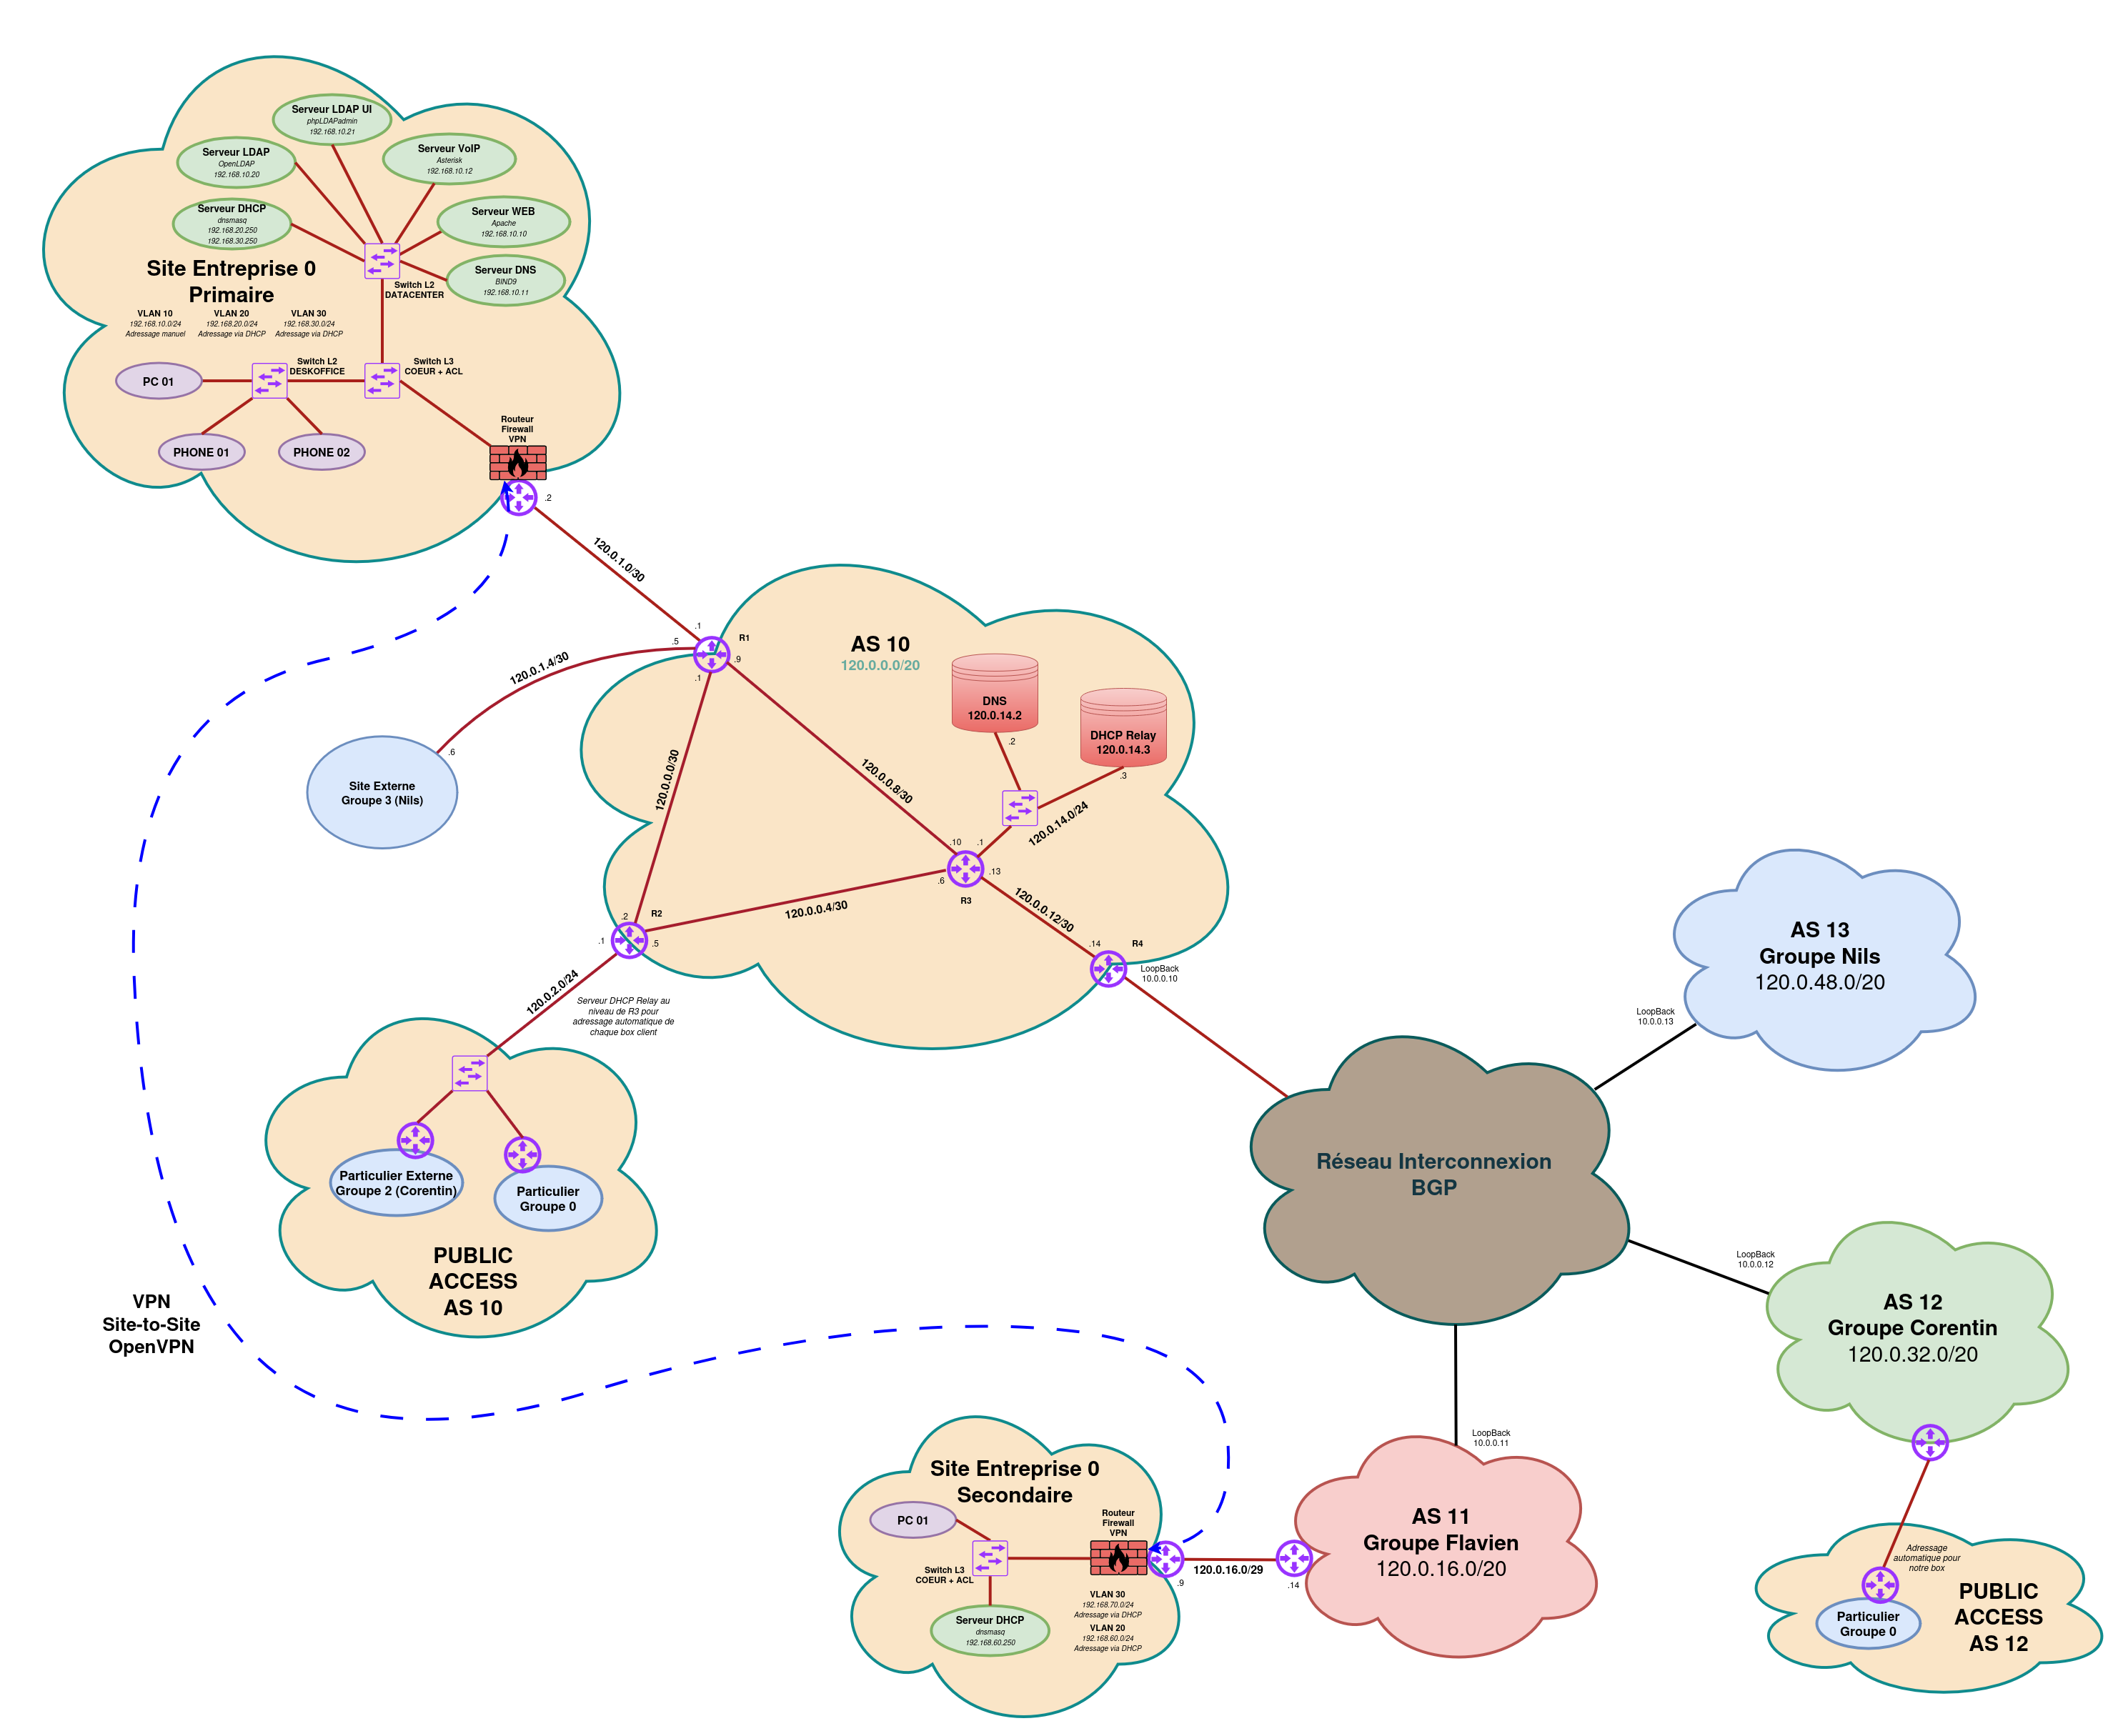
\includegraphics[width=1\linewidth]{image/schema_archi/ArchiGenerale.png}
    \caption{Schéma de l'architecture générale}
    \label{fig:schema_archi_generale}
\end{figure}

\subsection{Choix techniques}

\subsubsection{Routage interne}

Pour le routage interne de l'AS 10, nous avons choisi d'utiliser OSPF. Ce protocole permet aux routeurs d'échanger automatiquement les routes des différents sous-réseaux de l'infrastructure.\\

Tous les routeurs de l'AS participent à la même aire OSPF. Cela garantit un routage dynamique et évite d'avoir à modifier manuellement les tables de routage en cas de coupure d'un lien.\\

Les liens entre routeurs sont configurés en /30 afin de limiter le gaspillage d'adresses IP.

\subsubsection{Routage inter-AS}

La communication avec les autres systèmes autonomes est assurée par le protocole BGP.

Le routeur en bordure de l'AS établit des sessions BGP avec les AS voisins pour échanger les routes et assurer l'interconnexion avec les autres réseaux du projet.

\subsection{Services mis en place}

Plusieurs services ont été déployés dans l'infrastructure globale pour répondre aux exigences du projet. Ils se divisent en deux catégories selon qu'ils sont opérés par le fournisseur d'accès ou hébergés par l'entreprise cliente :

\paragraph{Services fournis par l'opérateur (AS 10) :}
\begin{itemize}
    \item Un service DHCP permettant d'attribuer automatiquement une adresse IP aux clients particuliers
    \item Un serveur DNS pour la résolution des noms de domaine entre les différents réseaux
    \item Un accès Internet via le routage BGP pour les entreprises clientes
\end{itemize}

\vspace{0.5cm}

\paragraph{Services hébergés par l'entreprise :}
\begin{itemize}
    \item Un serveur DNS interne gérant la zone locale de l'entreprise
    \item Un serveur Web hébergeant une page de test pour valider le filtrage réseau
    \item Un serveur LDAP pour la gestion centralisée des comptes utilisateurs et la sécurisation de l'accès VPN
    \item Un serveur Asterisk pour la téléphonie sur IP interne
\end{itemize}
